\documentclass[usenames,dvipsnames,svgnames,table,aspectratio=1610,mathserif]{beamer}

\mode<presentation> {

%\usetheme{default}
\usetheme{Madrid}

\setbeamertemplate{footline} % To remove the footer line in all slides uncomment this line

\setbeamertemplate{navigation symbols}{} % To remove the navigation symbols from the bottom of all slides uncomment this line
}

\usepackage{graphicx} % Allows including images
\usepackage{booktabs} % Allows the use of \toprule, \midrule and \bottomrule in tables
\usepackage{hyperref}
\usepackage{apacite}
\usepackage{fancyvrb}
\usepackage{color}
\usepackage{alltt}
\usepackage{listings}
\usepackage{framed}
\usepackage{courier}
\usepackage{minted}
\usepackage{epstopdf}
\usepackage{xifthen}
\usepackage[utf8]{inputenc}
\usepackage[T1]{fontenc}
\usepackage{textcomp}
\usepackage{gensymb}

\hypersetup{colorlinks=false}

\setbeamertemplate{bibliography entry title}{}
\setbeamertemplate{bibliography entry location}{}
\setbeamertemplate{bibliography entry note}{}
\setbeamertemplate{itemize items}[circle]
\setbeamertemplate{enumerate items}[circle]
\beamertemplatenavigationsymbolsempty
\setbeamertemplate{footline}{}

\newminted{haskell}{}
\newminted{java}{}
\newminted{scala}{}

\definecolor{g}{RGB}{0,100,0}
\newcommand{\highlight}[1]{\colorbox{yellow}{#1}}
\newcommand{\nega}[1]{\colorbox{yellow}{#1}}
\newcommand{\posi}[1]{\colorbox{green}{#1}}
\newcommand{\nl}{\vspace{\baselineskip}}
\newcommand{\pnl}{\pause \nl}

\newcommand{\textslide}[1]{{
\begin{frame}\begin{center}

#1

\end{center}\end{frame}
}}

\newcommand{\imageslide}[2][1]{{
\begin{frame}\begin{center}
\includegraphics[scale=#1]{#2}
\end{center}\end{frame}
}}

\newcommand{\imagetextslide}[3][1]{{
\begin{frame}\begin{center}

{#3}

\includegraphics[scale=#1]{#2}
\end{center}\end{frame}
}}

\newcommand{\ctof}{{
\LARGE $\degree F = \degree C \times \frac{9}{5} + 32$
}}

\newcommand{\ftoc}{{
\LARGE $\degree C = (\degree F - 32) \div \frac{9}{5}$
}}

%%----------------------------------------------------------------------------------------
%	TITLE PAGE
%----------------------------------------------------------------------------------------

\title[Propagators]{Propagators: An Introduction} % The short title appears at the bottom of every slide, the full title is only on the title page
\titlegraphic{
\includegraphics[scale=0.2]{data61.eps}}
\author{George Wilson} % Your name
\institute[] % Your institution as it will appear on the bottom of every slide, may be shorthand to save space
{
Data61/CSIRO\\ % Your institution for the title page
\medskip
\href{george.wilson@data61.csiro.au}{george.wilson@data61.csiro.au} % Your email address
}
\date{\today} % Date, can be changed to a custom date

\begin{document}


%%%%%
%%%%% Intro section
%%%%%


\begin{frame}
\titlepage % Print the title page as the first slide
\end{frame}


\begin{frame}

\begin{columns}
  \begin{column}{0.5\textwidth}
    \begin{center}
      
\includegraphics[scale=0.015]{what-are-birds.jpg}

      \nl

      What?
    \end{center}
  \end{column}
  \begin{column}{0.5\textwidth}
    \begin{center}
      
\includegraphics[scale=0.3]{for-what-purpose.jpg}

      \nl

      Why?
    \end{center}
  \end{column}
\end{columns}

\end{frame}


%%%%%
%%%%% History
%%%%%


\begin{frame}

\begin{columns}
\begin{column}{0.5\textwidth}
Roots as early as the 1970's at MIT
\begin{itemize}
  \item Guy L. Steele Jr. 
  \item Gerald J. Sussman
  \item Richard Stallman
\end{itemize}

\nl

More recently:
\begin{itemize}
  \item Alexey Radul
\end{itemize}
\end{column}
\begin{column}{0.5\textwidth}
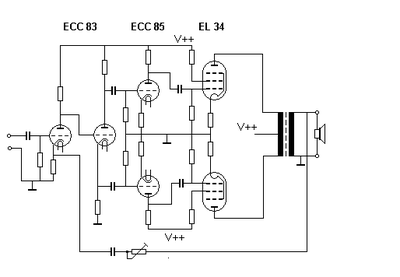
\includegraphics[scale=0.6]{circuit.png}
\end{column}
\end{columns}

\end{frame}


\begin{frame}[fragile]

\begin{verbatim}
(define (map f xs)
  (cond ((null? xs) '())
        (else (cons (f (car xs))
                    (map f (cdr xs)))))))
\end{verbatim}
\end{frame}


\begin{frame}
\begin{columns}
\begin{column}{0.005\textwidth}
\end{column}
\begin{column}{0.4\textwidth}
And then
\begin{itemize}
\item Edward Kmett
\end{itemize}
\nl
\nl

\includegraphics[scale=0.2]{haskell.png}
\end{column}
\begin{column}{0.5\textwidth}
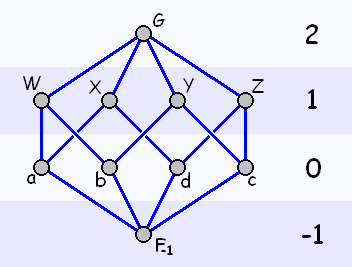
\includegraphics[scale=0.4]{hasse.png}

\nl
\nl

{\LARGE
  $x \le y \implies f(x) \le f(y)$
}
\end{column}
\end{columns}
\end{frame}


%%%%%
%%%%% What and why
%%%%%


\begin{frame}

\begin{center}
{\Huge Propagators}
\end{center}

\end{frame}


\begin{frame}
The {\it propagator model} is a model of computation

\nl

We model computations as {\it propagator networks}
\end{frame}


\begin{frame}

A propagator network comprises
\begin{itemize}
\item cells
\item propagators
\item connections between cells and propagators
\end{itemize}

\end{frame}


\imageslide{diagrams/cell1.pdf}
\imageslide{diagrams/cell2.pdf}
\imageslide{diagrams/prop.pdf}

%\imageslide{diagrams/always1.pdf}
%\imageslide{diagrams/always2.pdf}
%\imageslide{diagrams/always3.pdf}
%\imageslide{diagrams/always4.pdf}

\imageslide{diagrams/upper1.pdf}
\imageslide{diagrams/upper2.pdf}
\imageslide{diagrams/upper3.pdf}

\imageslide{diagrams/add1.pdf}
\imageslide{diagrams/add2.pdf}
\imageslide{diagrams/add3.pdf}
\imageslide{diagrams/add4.pdf}


%%%%% bidirectionality


\begin{frame}
  \begin{center}
    \begin{LARGE}
      $z \leftarrow x + y$
    \end{LARGE}
  \end{center}
\end{frame}


\begin{frame}
  \begin{center}
    \begin{LARGE}
      $z = x + y$
    \end{LARGE}
  \end{center}
\end{frame}


\begin{frame}
  \begin{center}
    \begin{LARGE}
      $7 = x + 4$
    \end{LARGE}
  \end{center}
\end{frame}


\begin{frame}
  \begin{center}
    \begin{LARGE}
      $7 = 3 + 4$
    \end{LARGE}
  \end{center}
\end{frame}


\begin{frame}
  \begin{center}
    \begin{LARGE}
      $z = x + y$
    \end{LARGE}
  \end{center}
\end{frame}


\begin{frame}
  \begin{center}
    \begin{LARGE}
      $z \leftarrow x + y$

      \nl

      $x \leftarrow z - y$

      \nl

      $y \leftarrow z - x$

    \end{LARGE}
  \end{center}
\end{frame}


\imageslide{diagrams/badd1.pdf}
\imageslide{diagrams/badd2.pdf}
\imageslide{diagrams/badd3.pdf}
\imageslide{diagrams/badd4.pdf}


\begin{frame}
\begin{center}
{\LARGE Propagators let us express multidirectional relationships!}
\end{center}
\end{frame}

\imagetextslide[0.8]{diagrams/celsius1.pdf}{\ctof}
\imagetextslide[0.8]{diagrams/celsius2.pdf}{\ctof}
\imagetextslide[0.8]{diagrams/celsius3.pdf}{\ctof}
\imagetextslide[0.8]{diagrams/celsius4.pdf}{\ctof}
\imagetextslide[0.65]{diagrams/celsius5.pdf}{\ctof \\ \nl \ftoc}
\imagetextslide[0.65]{diagrams/celsius6.pdf}{\ctof \\ \nl \ftoc}
\imagetextslide[0.65]{diagrams/celsius7.pdf}{\ctof \\ \nl \ftoc}
\imagetextslide[0.65]{diagrams/celsius8.pdf}{\ctof \\ \nl \ftoc}
\imagetextslide[0.65]{diagrams/celsius9.pdf}{\ctof \\ \nl \ftoc}
\imagetextslide[0.65]{diagrams/celsius10.pdf}{\ctof \\ \nl \ftoc}
\imagetextslide[0.65]{diagrams/celsius11.pdf}{\ctof \\ \nl \ftoc}
\imageslide[0.65]{diagrams/celsius12.pdf}
\imageslide[0.65]{diagrams/celsius13.pdf}
\imageslide[0.65]{diagrams/celsius14.pdf}
\imageslide[0.65]{diagrams/celsius15.pdf}
\imageslide[0.65]{diagrams/celsius16.pdf}

\textslide{\Large{We can combine networks into larger networks!}}

%%%%% partiality


\textslide{{\LARGE
What types are the values of the cells?
}}


\imageslide{diagrams/cell3.pdf}
\imageslide{diagrams/cell2.pdf}
\imageslide{diagrams/cell1.pdf}


\textslide{{\LARGE
  {\tt data Maybe a = Nothing | Just a}
}}


\imageslide{diagrams/always1.pdf}
\imageslide{diagrams/always2.pdf}
\imageslide{diagrams/always3.pdf}
\imageslide{diagrams/always4.pdf}
\imageslide{diagrams/contradiction1.pdf}
\imageslide{diagrams/contradiction2.pdf}
\imageslide{diagrams/contradiction3.pdf}

\textslide{{\Huge \bf
:(

\nl
}

\LARGE{Contradiction}

}


\begin{frame}[fragile]

\begin{haskellcode}
data Perhaps a = Unknown | Known a | Contradiction
\end{haskellcode}

\pnl

\begin{haskellcode}
instance Eq a => Monoid (Perhaps a) where
  mempty = Unknown

  mappend Unknown x           = x
  mappend x       Unknown     = x
  mappend Contradiction _     = Contradiction
  mappend _     Contradiction = Contradiction
  mappend (Known a) (Known b) =
    if a == b
      then Known a
      else Contradiction
\end{haskellcode}

\end{frame}

\textslide{\LARGE Partial information!}


\textslide{\LARGE ?}

\begin{frame}
\begin{center}
\Huge $[1,5]$
\end{center}
\end{frame}


\begin{frame}
\begin{center}
\Huge $[1, 5] <> [2, 7] = [2,5]$
\end{center}
\end{frame}


\begin{frame}
\begin{center}
\Huge $\{True,\ False\}$
\end{center}
\end{frame}


\begin{frame}
TODO set intersection examples
\end{frame}


\end{document} 

